\documentclass[12pt]{article}
\usepackage[utf8]{inputenc}
\usepackage[T1]{fontenc}
\usepackage{amsmath}
\usepackage{amsfonts}
\usepackage{amssymb}
\usepackage[version=4]{mhchem}
\usepackage{stmaryrd}
\usepackage{physics}
\usepackage{graphicx}


\usepackage{listings} % Required for insertion of code
\usepackage{xcolor} % Required for custom colors

% Define custom colors
\definecolor{codegreen}{rgb}{0,0.6,0}
\definecolor{codegray}{rgb}{0.5,0.5,0.5}
\definecolor{codepurple}{rgb}{0.58,0,0.82}
\definecolor{backcolour}{rgb}{0.95,0.95,0.92}

% Setup the style for code listings
\lstdefinestyle{mystyle}{
    backgroundcolor=\color{backcolour},   
    commentstyle=\color{codegreen},
    keywordstyle=\color{magenta},
    numberstyle=\tiny\color{codegray},
    stringstyle=\color{codepurple},
    basicstyle=\ttfamily\footnotesize,
    breakatwhitespace=false,         
    breaklines=true,                 
    captionpos=b,                    
    keepspaces=true,                 
    numbers=left,                    
    numbersep=5pt,                  
    showspaces=false,                
    showstringspaces=false,
    showtabs=false,                  
    tabsize=2
}

% Activate the style
\lstset{style=mystyle}


\title{Ch14 Winter term 2024 }

\author{}
\date{}


\begin{document}
\maketitle
Problem set 3

due April 25, 2024

unless otherwise stated, assume $\mathrm{T}=25^{\circ} \mathrm{C}$, that activities = concentrations and $\mathrm{K}_{\mathrm{w}}=10^{-14}$. unless otherwise specified, give answers to 3 significant figures.

\section{}
The ion product of water, $\mathrm{K}^{\circ}$, is defined as the product of the activities of $\mathrm{H}^{+}$and $\mathrm{OH}^{-}$in pure water. At $298 \mathrm{~K}, K_{W}^{\circ}=a_{\mathrm{H}^{+}} a_{\mathrm{OH}^{-}}=1.00 \times 10^{-14}$. In pure water (ionic strength 0), activities and concentrations are equivalent. Due to charge balance considerations, the concentration of $\left(\mathrm{H}^{+}\right)$must equal the concentration of $\left(\mathrm{OH}^{-}\right)$in pure water, so that $\left(H^{+}\right)=a_{H^{+}}=\sqrt{K_{w}^{\circ}}=10^{-7} \mathrm{M}$.\\
The concentration constant, $\mathrm{K}_{\mathrm{w}}$, is defined as the product of the concentrations of $\mathrm{H}^{+}$and $\mathrm{OH}^{-}$:

$$
K_{W}=\left(H^{+}\right)\left(O H^{-}\right)=K_{W}^{\circ} /\left(\gamma_{H^{+}} \gamma_{O H^{-}}\right)
$$

What is the concentration of $\mathrm{H}^{+}$in an aqueous solution of $0.15 \mathrm{M} \mathrm{NaCl}$ at $298 \mathrm{~K}$ ? Assume that the Debye-Hückel limiting law is valid for the activity coefficients of $\mathrm{H}^{+}$and $\mathrm{OH}^{-}$ions at this ionic strength.

The contributions of $\mathrm{H}^{+}$and $\mathrm{OH}^{-}$to the ionic strength can be neglected.

\subsection{Answer}
The formula for calculating an ionic strength is given by:
\begin{equation}
  I=\frac{1}{2} \sum_{i} c_{i} z_{i}^{2}
\end{equation}
where $c_{i}$ is the concentration of the $i$th ion and $z_{i}$ is the charge of the $i$th ion. In this case, the ionic strength is given by:
\begin{equation}
  I=\frac{1}{2}\left(0.15 \times 1^{2}+0.15 \times 1^{2}\right)=0.15
\end{equation}
The Debye-Hückel limiting law is given by:
\begin{equation}
  \log \gamma_{\pm}=-0.509 z_{+} z_{-} \sqrt{I}
\end{equation}
where the solvent is water at $298 \mathrm{~K}$, $z_{+}$ and $z_{-}$ are the charges of the cation and anion, respectively, and $I$ is the ionic strength. Since the charges of $\mathrm{H}^{+}$ and $\mathrm{OH}^{-}$ are both 1, the activity coefficients are the same.
Now, with knowledge of the activity coefficients, we can use the given equation for the concentration constant of water to find the concentration of $\mathrm{H}^{+}$.
% Inline Python code in the document
\begin{lstlisting}[language=Python]
from sympy import symbols, Eq, sqrt, log, solve

# Define symbols
I, gamma_pm, Kw, Kwo, c_Hp, c_OHm = symbols('I gamma_pm K_w K_wo c_H+ c_OH-')

# Constants and given values
Kwo_value = 1.00e-14  # Standard ion product of water at 298 K
A = 0.5085  # Debye-Huckel constant for water at 298 K
c_NaCl = 0.15  # Concentration of NaCl

# Ionic strength calculation
I_value = 0.5 * (c_NaCl * 1**2 + c_NaCl * 1**2)  # Sum of 0.15 * 1^2 + 0.15 * 1^2

# Debye-Huckel equation for activity coefficients
log_gamma_pm = -A * sqrt(I_value)

# Converting log_gamma to actual gamma
gamma_pm_value = 10**log_gamma_pm

# Ion product of water considering activity
Kw_eq = Eq(Kw, Kwo / (gamma_pm_value**2))

# Solve for H+ concentration assuming (H+) = (OH-)
c_Hp_eq = Eq(c_Hp**2, solve(Kw_eq, Kw)[0])
c_Hp_value = solve(c_Hp_eq, c_Hp)

c_Hp_value
\end{lstlisting}
This gives us $\mathrm{H}^{+}= \pm 1.574 \times \sqrt{K_W^{\circ}}$. Since the concentration of $\mathrm{H}^{+}$ cannot be negative, we take the positive value and we plug in for $\sqrt{K_W^{\circ}}$ to get $\mathrm{H}^{+}=1.57 \times 10^{-7} \mathrm{M}$.
% Inline Python code in the document
\begin{lstlisting}[language=Python]
from sympy import sqrt

# Redefine the concentration of H+ using the positive root and substituting Kwo_value
c_Hp_final = 1.57376978563008 * sqrt(Kwo_value)

c_Hp_final.evalf()
\end{lstlisting}

\section{}
Phosphate Buffered Saline (PBS) is often used in biochemical studies since it mimics physiological pH and ionic strength. A variant of PBS is prepared that has the following composition

\begin{center}
\begin{tabular}{|l|l|}
\hline
compound & $M$ \\
\hline
$\mathrm{NaCl}$ & 0.150 \\
\hline
$\mathrm{K}_{2} \mathrm{HPO}_{4}$ & 0.010 \\
\hline
$\mathrm{KH}_{2} \mathrm{PO}_{4}$ & 0.0020 \\
\hline
\end{tabular}
\end{center}

The pKa of $\mathrm{H}_{2} \mathrm{PO}_{4}^{-}$is 7.20 . These salts can be assumed to be fully dissociated into their constituent ions $\left(\mathrm{Na}^{+}, \mathrm{Cl}^{-}, \mathrm{K}^{+}, \mathrm{HPO}_{4}{ }^{2-}\right.$ and $\left.\mathrm{H}_{2} \mathrm{PO}_{4}^{-}\right)$, and the temperature is $25^{\circ} \mathrm{C}$.

\subsection{}
Neglecting ionic strength effects on the activity coefficients, what is the $\mathrm{pH}$ of this solution? You can use the Henderson-Hasselbalch equation for this calculation. Even though there are potentially 4 different phosphate species, the contributions of $\mathrm{H}_{3} \mathrm{PO}_{4}$ and $\mathrm{PO}_{4}{ }^{3-}$ ions to the $\mathrm{pH}$ calculation can be neglected since they are present at very low concentrations.
\subsubsection{Answer}
We know that the instruction to neglect the ionic strength means that we can neglect $\mathrm{NaCl}$ for the purposes of this calculation. The dissociation of $\mathrm{K}_{2} \mathrm{HPO}_{4}$ and $\mathrm{KH}_{2} \mathrm{PO}_{4}$ will make the concentrations of $\mathrm{HPO}_{4}{ }^{2-}$ and $\mathrm{H}_{2} \mathrm{PO}_{4}^{-}$ equal to $0.010$ and $0.0020$ M, respectively. We recognize that these are a pair of a conjugate base and an acid, respectively, with the $\mathrm{pK}_{a}$ of $\mathrm{H}_{2} \mathrm{PO}_{4}^{-}$ being $7.20$.
The Henderson-Hasselbalch equation is given by:
\begin{equation}
  \mathrm{pH}=\mathrm{pK}_{a}+\log \left(\frac{[\text { CB }]}{[\text { ACID }]}\right)
\end{equation}
% Inline Python code in the document
\begin{lstlisting}[language=Python]
pKa_H2PO4 = 7.20  # pKa for H2PO4^-
conjugate_base_concentration = 0.010  # [HPO4^{2-}]
acid_concentration = 0.0020  # [H2PO4^-]

# Calculate pH using the Henderson-Hasselbalch equation
phosphate_buffer_pH = pKa_H2PO4 + math.log10(conjugate_base_concentration / acid_concentration)
phosphate_buffer_pH
\end{lstlisting}
This gives us a $\mathrm{pH}$ of $7.90$ for the solution.
\subsection{}

For charged species like $\mathrm{HPO}_{4}{ }^{2-}$ and $\mathrm{H}_{2} \mathrm{PO}_{4}$, however, it can be problematic neglecting ionic strength effects, since activity coefficients vary with ionic strength. What is the $\mathrm{pH}$ of this solution, including ionic strength effects? Use the Debye Hückel limiting law to evaluate the ionic strength dependence of the activity coefficients. The contributions of $\mathrm{H}^{+}$and $\mathrm{OH}^{-}$to the ionic strength can be neglected.
\subsubsection{Answer}
First, we want to compute the concentrations of each ion:
\begin{equation}
  \begin{aligned}
    \text { For } \mathrm{NaCl} & : \text { } [\mathrm{Na}^{+}]=0.150 \text { and } [\mathrm{Cl}^{-}]=0.150 \\
    \text { For } \mathrm{K}_{2} \mathrm{HPO}_{4} & : [\mathrm{HPO}_{4}{ }^{2-}]=0.010 \mathrm{M} \\
    \text { For } \mathrm{KH}_{2} \mathrm{PO}_{4} & : \text { } [\mathrm{H}_{2} \mathrm{PO}_{4}^{-}]=0.0020 \mathrm{M}
  \end{aligned}
\end{equation}
the concentration of potassium is given by the contribution from $\mathrm{K}_{2} \mathrm{HPO}_{4}$ and $\mathrm{KH}_{2} \mathrm{PO}_{4}$:
\begin{equation}
  [\mathrm{K}^{+}]=2 \times 0.010+0.0020=0.0220 \mathrm{M}
\end{equation}
We use the formula for organic strength again which was given by:
\begin{equation}
  I=\frac{1}{2} \sum_{i} c_{i} z_{i}^{2}
\end{equation}
We can use the concentrations to compute the ionic strength as $0.182 \mathrm{M}$.
% Inline Python code in the document
\begin{lstlisting}[language=Python]
# Define the concentrations and charges of ions
Na_plus = 0.150
Cl_minus = 0.150
K_plus = 0.022  # Sum of K+ from both salts
HPO4_2minus = 0.010
H2PO4_minus = 0.0020

# Ionic strength calculation
ionic_strength = 0.5 * (Na_plus * 1**2 + Cl_minus * 1**2 + K_plus * 1**2 + HPO4_2minus * 2**2 + H2PO4_minus * 1**2)
ionic_strength
\end{lstlisting}

The Debye-Hückel limiting law is given by:
\begin{equation}
  \log \gamma=-0.509 z^{2} \sqrt{I}
\end{equation}
We use this to calculate the activity coefficients for the $\mathrm{HPO}_{4}^{2-}$ and $\mathrm{H}_{2}\mathrm{PO}_{4}^{-}$ ions.
% Inline Python code in the document
\begin{lstlisting}[language=Python]
import math

# Redefining constants and ionic strength value as the session reset
A = 0.5085
ionic_strength_value = 0.182

# Charges of the ions
z_HPO4_2minus = -2
z_H2PO4_minus = -1

# Calculate activity coefficients using Debye-Huckel limiting law
log_gamma_HPO4_2minus = -A * (z_HPO4_2minus**2) * math.sqrt(ionic_strength_value)
log_gamma_H2PO4_minus = -A * (z_H2PO4_minus**2) * math.sqrt(ionic_strength_value)

# Convert log to actual coefficients
gamma_HPO4_2minus = 10**log_gamma_HPO4_2minus
gamma_H2PO4_minus = 10**log_gamma_H2PO4_minus

log_gamma_HPO4_2minus, log_gamma_H2PO4_minus, gamma_HPO4_2minus, gamma_H2PO4_minus
\end{lstlisting}
So, for the activity coefficients of $\mathrm{HPO}_{4}^{2-}$, $\gamma_{HPO_{4}^{2-}}=0.136$ and for $\mathrm{H}_{2}\mathrm{PO}_{4}^{-}$, $\gamma_{H_{2}PO_{4}^{-}}=0.607$.
Now the modified Henderson-Hasselbalch equation is going to be given by:
\begin{equation}
  \mathrm{pH}=\mathrm{pK}_{a}+\log \left(\frac{[HPO_{4}^{2-}] \times \gamma_{HPO_{4}^{2-}}}{[H_{2}PO_{4}^{-}] \times \gamma_{H_{2}PO_{4}^{-}}}\right)
\end{equation}
Calculating and obtaining the $\mathrm{pH}$ of the solution as $7.25$.
% Inline Python code in the document
\begin{lstlisting}[language=Python]
# Given pKa and concentrations
pKa_H2PO4 = 7.20
concentration_HPO4_2minus = 0.010  # Molar concentration of HPO4^{2-}
concentration_H2PO4_minus = 0.0020  # Molar concentration of H2PO4^-

# Calculate the pH using adjusted concentrations with activity coefficients
phosphate_buffer_pH_adjusted = pKa_H2PO4 + math.log10(
    (concentration_HPO4_2minus * gamma_HPO4_2minus) / (concentration_H2PO4_minus * gamma_H2PO4_minus)
)

phosphate_buffer_pH_adjusted
\end{lstlisting}

\section{}
The pKas for 1,3-diaminopropane are $\mathrm{pK}_{\mathrm{a} 1}=8.29$ and $\mathrm{pK}_{\mathrm{a} 2}=10.30$. Which of these two pKas do you expect to most closely resemble the pKa of 1-aminopropane? Explain briefly. Remember that acid dissociation constants are defined starting with the fully protonated species.
\subsection{Answer}
The chemical structures are given by:\\
\begin{figure}[h]
  \centering
  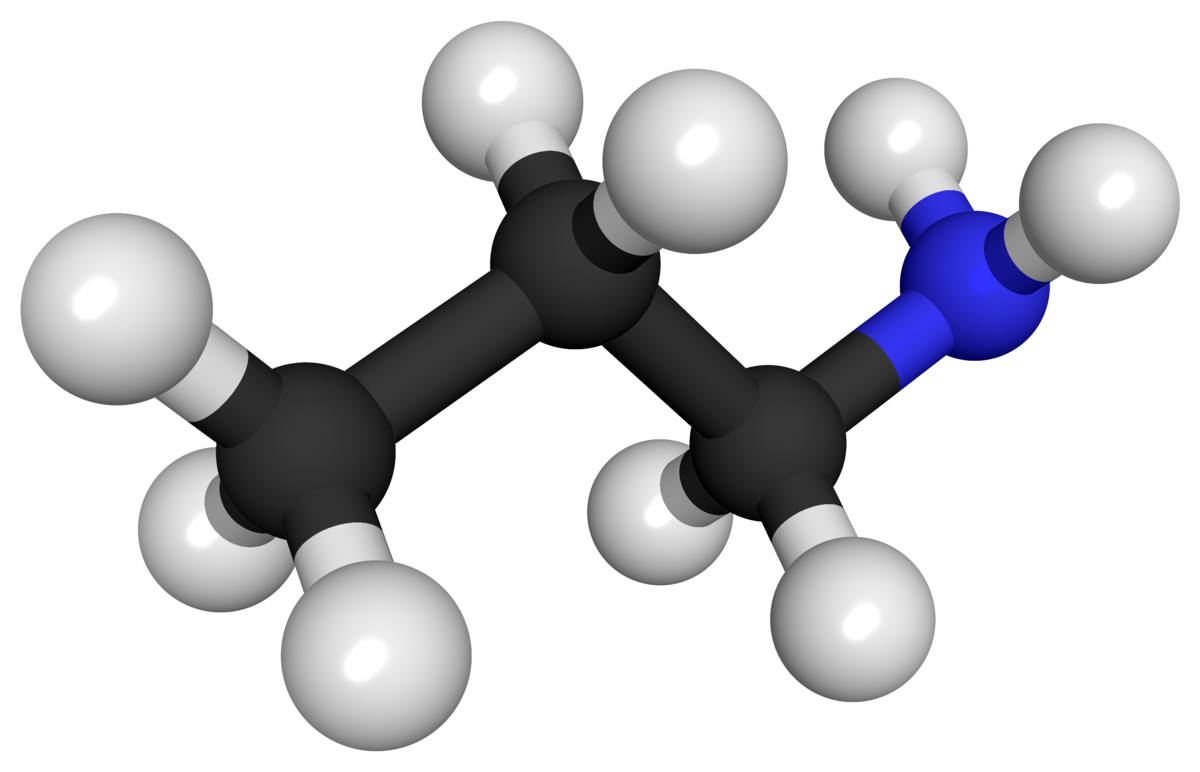
\includegraphics[width=\textwidth]{amine.png}
  \caption{1-aminopropane}
\end{figure}
\begin{figure}[h]
  \centering
  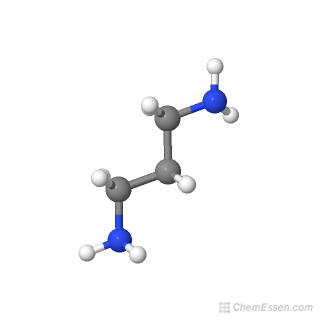
\includegraphics[width=\textwidth]{dia.png}
  \caption{1,3-diaminopropane}
\end{figure}
I would expect the first pKa of 1,3-diaminopropane ($\mathrm{pK}_{\mathrm{a} 1}$) to most closely resemble the pKa of 1-aminopropane. I think the conjugate base for the first dissociation of 1,3-diaminopropane has a similar stability to the conjugate base of 1-aminopropane. This situation would be different if there was a pi system along the alkyl chain, to better stabilize the positive charge on the nitrogen, but there isn't.
\newpage
\section{}
A buffer solution with malonic acid was prepared by adding 0.05 moles of malonic acid ($\mathrm{HOOC}-\mathrm{CH}_{2}-\mathrm{COOH}$) and 0.1 mole of $\mathrm{Na}_{2}$ malonate ($\mathrm{Na}^{+}-\mathrm{OOC}-\mathrm{CH}_{2}-\mathrm{COO}^{-}\mathrm{Na}^{+}$) to make an aqueous solution with a total volume $=1$ liter. The pKas for malonic acid are $\mathrm{pKa}_{1}=2.83$ and $\mathrm{pKa}_{2}=5.69$. Calculate the $\mathrm{pH}$ of this solution. 


Note: $(\mathrm{H}^{+})$ and $(\mathrm{OH}^{-})$ can be neglected in the charge balance equation since they have significantly smaller concentrations than the other charged species. You can also assume activities equal concentrations in working on this problem. With these approximations, the $\mathrm{pH}$ can be calculated by solving a quadratic equation so that it is not necessary to use Mathematica$^{\circledR}$, etc. for this problem - but you certainly can.
\subsection{Answer}
We know that there are two sources for the malonate ion, so we can define a mass balance equation as:
\begin{equation}
  c_{T}=c_1+c_2
=\end{equation}
where we define $c_{T}$ as the total concentration of malonate, $c_1$ as the concentration of malonic acid, and $c_2$ as the concentration of malonate. 
And then we also know that the total concentration of sodium ions will be given by $2c_2$. Now, we consider the equilibrium equations for the acids:
\begin{equation}
  Ka_{1}=\frac{[H^{+}][HA^{-}]}{[H_2A]}
\end{equation}
\begin{equation}
  Ka_{2}=\frac{[H^{+}][A^{2-}]}{[HA^{-}]}
\end{equation}
where $A^{2-}$ is the malonate ion and $HA^{-}$ is malonic acid.
We can then substitute the concentrations of these species into the mass balance equation, which will allow us to get expressions for $[HA^{-}]$ and $[A^{2-}]$ in terms of $c_{T}$, $Ka_{1}$, and $Ka_{2}$ and $[H^{+}]$. Next, we want to consider the charge balance equation:
\begin{equation}
  [H^{+}] + [Na^{+}] = [HA^{-}] + 2[A^{2-}] + [OH^{-}]
\end{equation}
This allows us to get to:
\begin{equation}
[H^+]+2 c_2=c_T \frac{K_1[H^+]+2 K_1 K_2}{[H^+]^2+K_1[H^+]+K_1 K_2}+\frac{K_w}{[H^+]}
\end{equation}
where $K_w$ is the ion product of water. At this point we can follow the instruction to neglect the concentrations of $(H^{+})$ and $(OH^{-})$ in the charge balance equation. This eventually gives the proton concentration as:
\begin{equation}
[H^+]=\sqrt{K_1 K_2}
\end{equation}
Giving a $\mathrm{pH}$ of $4.26$.
\begin{equation}
\mathrm{pH}=-\log_{10}(\sqrt{K_1 K_2})
\end{equation}
% Inline Python code in the document
\begin{lstlisting}[language=Python]
from sympy import symbols, sqrt, log

# Define the constants
Ka1, Ka2, Kw = symbols('Ka1 Ka2 Kw', real=True, positive=True)
pKa1, pKa2 = 2.83, 5.69  # Given pKa values

# Convert pKa to Ka
Ka1_value = 10**(-pKa1)
Ka2_value = 10**(-pKa2)
Kw_value = 10**(-14)  # Ion product of water at 25 C

# Calculating [H+] using the square root of the product of the dissociation constants
H_plus = sqrt(Ka1_value * Ka2_value)

# Calculate pH from [H+]
pH_value = -log(H_plus, 10)

# Evaluate the expression for pH
final_pH = pH_value.evalf()
final_pH

\end{lstlisting}
\end{document}